% University of Glasgow School of Computing Science project template
% Dissertation outline for MSc project planning.
\documentclass{l4proj}

\usepackage{pdfpages}

\begin{document}

%==============================================================================
%% METADATA
\title{Evaluating Open-Vocabulary Vision-Language Models for 2D Robotic Grasp Detection}
\author{Pang Zhenkun}
\date{MSc Robotics \& Artificial Intelligence\\Supervisor: Dr Jan Paul Siebert\\2026}

\maketitle

%==============================================================================
%% ABSTRACT
\begin{abstract}
    \todo{300--400 words. Summarise: (1) research background and problem, (2) methodology, including Cornell dataset, VLM grounding, and geometric grasp estimation, (3) key findings, and (4) implications or outcomes. Write this after the experiments are complete.}
\end{abstract}

%==============================================================================
%% ACKNOWLEDGEMENTS
\chapter*{Acknowledgements}
\todo{Add acknowledgements before final submission.}

%==============================================================================
%% EDUCATION REUSE CONSENT FORM
% Uncomment and complete these lines only if you consent to educational reuse.
%\def\consentname {Pang Zhenkun}
%\def\consentdate {Date}
\educationalconsent

%==============================================================================
\tableofcontents

%==============================================================================
\chapter{Introduction}
\pagenumbering{arabic}

\section{Background and Motivation}
\todo{About 3--5 paragraphs. Introduce robotic grasp detection, visual perception, and VLM/open-vocabulary grounding. Explain the current problem and why it remains unresolved or worth studying. Then state the theoretical and practical motivation for the project.}

\section{Research Questions}
\todo{State the main research question and supporting sub-questions. Explain why these questions matter for robotic perception and grasp detection.}

\section{Research Aim and Objectives}
\todo{State the overall aim of the project, then list concrete objectives such as dataset preparation, baseline implementation, VLM-assisted pipeline design, evaluation, and failure case analysis.}

\section{Scope of the Project}
\todo{Clarify boundaries: this project focuses on offline 2D grasp perception on Cornell, not physical robot control or full manipulation. State optional parts such as few-shot adaptation as extensions rather than core requirements.}

\section{Dissertation Structure}
\todo{Briefly describe the remaining chapters.}

%==============================================================================
\chapter{Literature Review}

\section{Robotic Grasp Detection}
\todo{Review prior research on robotic grasp detection. Explain how grasp detection is commonly formulated and why visual perception is central to this problem.}

\section{2D Grasp Rectangle Detection and Cornell Benchmarking}
\todo{Review the 2D grasp rectangle formulation and Cornell-style benchmarking. Include classic works such as Lenz et al. and Redmon and Angelova.}

\section{Classical Computer Vision and Deep Learning Approaches}
\todo{Summarise traditional CV methods and supervised deep learning methods. Critically compare their strengths and weaknesses, especially data dependence, generalisation, and interpretability.}

\section{Vision-Language Models and Open-Vocabulary Grounding}
\todo{Review VLMs, zero-shot/open-vocabulary perception, and grounding models such as Grounding DINO, OWL-ViT, or Florence-2. Focus on how these models may support object localisation for robotic perception.}

\section{Few-Shot and Lightweight Adaptation}
\todo{Briefly review optional adaptation methods such as LoRA or QLoRA. Explain why this is treated as an extension rather than the main project goal.}

\section{Literature Gap}
\todo{Critically identify limitations in previous work and explain the gap addressed by this dissertation: whether open-vocabulary grounding outputs can be converted into useful 2D robotic grasp rectangles through geometric post-processing.}

%==============================================================================
\chapter{Methodology}

\section{Research Design}
This dissertation uses a controlled, dataset-based experiment to examine where
open-vocabulary localisation is useful in a 2D grasp detection pipeline. No
human participants or questionnaire data are involved. Three systems are
evaluated. The first is a traditional computer-vision (CV) baseline that
operates on the complete image. The second uses Grounding DINO to localise an
object and applies a deterministic geometric grasp estimator within the
localised region. The third keeps the same Grounding DINO front end but replaces
the geometric estimator with a lightweight supervised CNN.

This design separates two questions that would otherwise be confounded:
whether language-conditioned localisation improves over whole-image
segmentation, and whether a learned grasp backend improves over a geometric
backend when both receive the same object crop. All three systems use the same
Cornell annotations and the same rectangle success criterion. The study is an
offline perception evaluation; it does not claim that a successful rectangle
necessarily produces a successful physical grasp.

\section{Cornell Dataset and Fixed Directory Split}
The experiments use all 885 RGB images in the Cornell Grasping Dataset. Each
sample contains one RGB image and multiple positively labelled grasp
rectangles. The shared data loader parses the four corner points of every
positive rectangle, associates them with the corresponding image, and converts
them to a common centre representation for evaluation. Although depth images
are available in Cornell, all three systems in this study use RGB so that input
modality is held constant.

For CNN development, Cornell directories 01--06 form the training set (600
images), directories 07--08 form the validation set (200 images), and
directories 09--10 form the fixed test subset (85 images). Directory membership
is used to reduce direct overlap between development and test data. This is a
project-specific split, not the standard image-wise or object-wise five-fold
protocol reported in prior Cornell studies. It is therefore described as a
\emph{fixed 85-sample test subset} rather than as a general unseen-object
benchmark.

\begin{figure}[htbp]
  \centering
  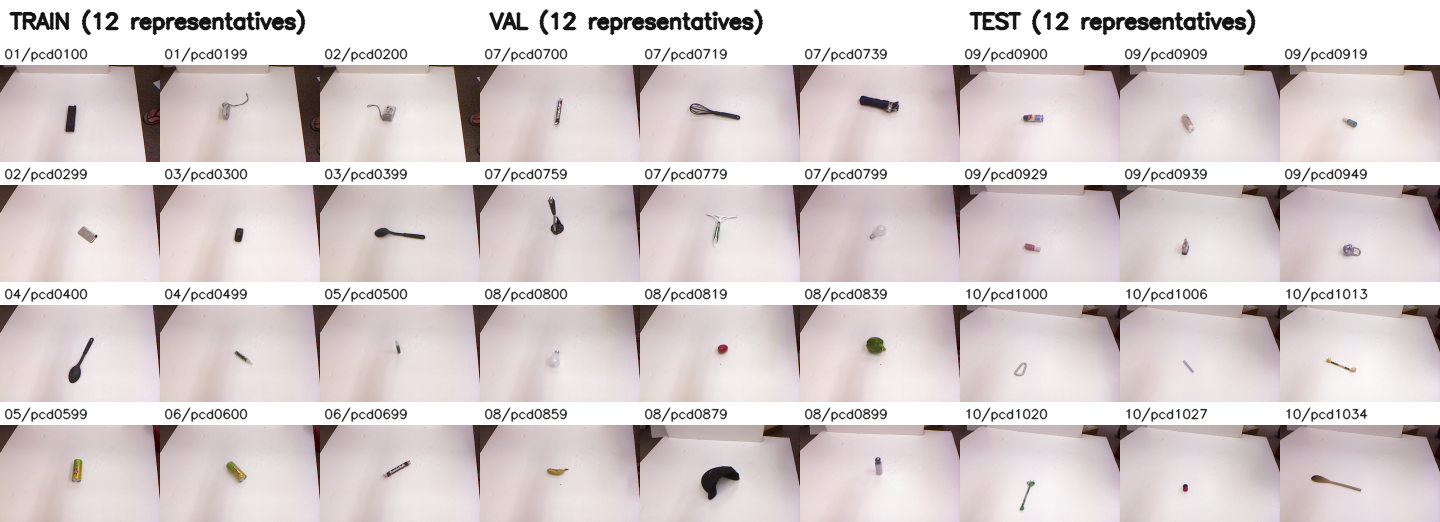
\includegraphics[width=\linewidth]{images/cornell_split_contact_sheet.png}
  \caption{Representative Cornell images from the training, validation, and
  fixed test directories. Twelve images were selected from each split, with
  directory-balanced sampling where possible. The figure documents visible
  object variation but cannot establish that the three splits have equal
  difficulty.}
  \label{fig:cornell-splits}
\end{figure}

\section{2D Grasp Rectangle Representation}
A grasp is represented as
\[
g=(c_x,c_y,w,h,\theta),
\]
where $(c_x,c_y)$ is the rectangle centre, $w$ and $h$ are its dimensions, and
$\theta$ is the in-plane gripper orientation. This follows the rectangle
representation introduced for RGB-D grasp detection by
\citet{jiang2011efficient} and used in subsequent Cornell work
\citep{lenz2015deep,redmon2015real}. Multiple positive rectangles may be
associated with an image. A prediction is compared with every positive
annotation, and the annotation with the highest intersection over union (IoU)
is used for scoring.

\section{Traditional Computer Vision Baseline}
The baseline applies colour and brightness thresholding to the complete RGB
image, cleans the binary mask, and extracts external contours. Contours smaller
than 80 pixels or touching an eight-pixel image boundary are rejected. The
remaining contour score favours large regions near the image centre. A
minimum-area rotated rectangle supplies the object centre and principal axes.
The grasp orientation is set perpendicular to the object's long axis. The
predicted grasp width is $1.35$ times the object short side, clipped to
20--120 pixels, and the height is $0.55$ times the short side, clipped to
15--45 pixels.

This method is deliberately simple and deterministic. It provides a
reproducible reference for measuring the value of localisation, but its
thresholds and size rules are engineering heuristics rather than learned
affordances.

\section{Grounding DINO Localisation Front End}
The two VLM-guided systems use Grounding DINO, an open-set detector that aligns
text and image features \citep{liu2023grounding}. Every image receives the same
generic prompt, \texttt{small object}, rather than a hand-written object name.
The box and text thresholds are both 0.25. Using one prompt for the complete
dataset avoids supplying sample-specific class information. The highest-ranked
valid box is retained and expanded by 10\% before grasp estimation to reduce
the risk of clipping the object boundary. The saved localisation run produced a
box for all 885 evaluated images.

\section{VLM-Guided Geometric Backend}
The geometric backend reuses the baseline's mask and contour operations, but
restricts the mask to the expanded Grounding DINO box. The largest suitable
local contour is converted to a grasp with the same minimum-area rectangle and
short-side rules used by the baseline. Consequently, the difference between
these two systems is principally the localisation front end. A box-derived
fallback is implemented for missing contours, although the evaluated run did
not require it.

\section{VLM-Guided Lightweight CNN Backend}
The learned backend receives the same expanded VLM crop, resized to
$224\times224$ RGB and normalised using ImageNet channel statistics. It predicts
one local grasp because localisation has already isolated the target. The
network contains four convolution--batch-normalisation--ReLU blocks with
32, 64, 128, and 256 channels. Spatial resolution is reduced by a stride-two
first convolution and max pooling. Adaptive global average pooling (GAP)
produces a 256-dimensional vector, followed by fully connected layers of 128
and 64 units and a six-dimensional output.

\begin{figure}[htbp]
  \centering
  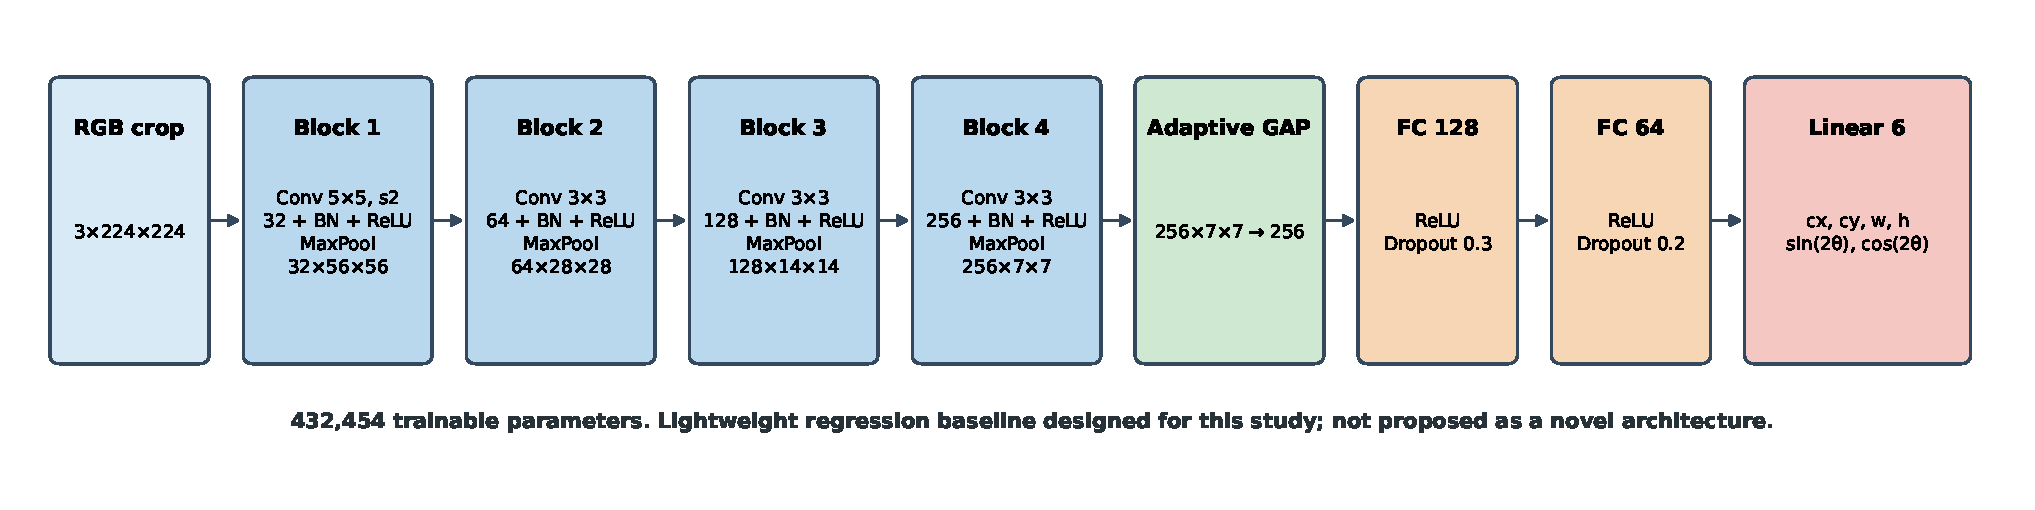
\includegraphics[width=\linewidth]{images/cnn_architecture.pdf}
  \caption{Lightweight CNN grasp regression baseline used in this study. The
  complete architecture is an engineering design for the controlled
  comparison and is not proposed as a novel grasp network.}
  \label{fig:cnn-architecture}
\end{figure}

The outputs are
$[c_x,c_y,w,h,\sin(2\theta),\cos(2\theta)]$. The double-angle representation
follows the symmetry-aware formulation used by GG-CNN
\citep{morrison2018closing}: for a parallel-jaw gripper, orientations separated
by 180 degrees are equivalent. The architecture has 432,454 trainable
parameters. Its complete layer schedule was not copied from one publication.
The light channel count and GAP were selected to limit overfitting and parameter
growth on the 600-image training split. The rectangle task is grounded in prior
Cornell work, while the exact four blocks and fully connected widths are
project-specific engineering choices.

\section{Training Protocol and Repeated Runs}
For each image, the largest-area positive rectangle whose centre lies in the
VLM crop supplies the regression target. Centre coordinates are normalised by
crop dimensions; width and height are normalised by the crop diagonal.
Optimisation uses Smooth L1 loss, Adam with learning rate $10^{-3}$ and weight
decay $10^{-4}$, batch size 32, and at most 80 epochs. A
ReduceLROnPlateau scheduler halves the learning rate after eight epochs without
validation improvement. Training stops after 20 epochs without a lower
validation loss, and the lowest-loss validation checkpoint is restored.

The experiment is repeated five times with seeds 42--46. For each run, the
selected checkpoint is evaluated over all 885 images and separately on
directories 09--10. Results are reported as population mean and standard
deviation across the five runs. The saved per-sample prediction file belongs to
the final run (seed 46) and is used only for matched-sample and qualitative
analysis.

\section{Cornell Rectangle Evaluation}
For prediction $P$ and ground-truth rectangle $G$, IoU is
\[
\operatorname{IoU}(P,G)=\frac{|P\cap G|}{|P\cup G|}.
\]
A prediction is successful if its best ground-truth match has
$\operatorname{IoU}\geq0.25$ and its parallel-gripper angle error is at most
$30^\circ$. Mean best IoU and mean best angle error are also reported, since
the binary success rate can hide whether failure is caused mainly by position,
size, or orientation. Whole-dataset results characterise the implemented
pipelines. Backend comparison is restricted to the same 85 test images so that
the geometric and CNN outputs are paired sample by sample.

\section{Methodological Limitations}
The directory split is not a standard Cornell five-fold protocol, and the
contact sheet in Figure~\ref{fig:cornell-splits} cannot prove equal shape or
difficulty distributions. The fixed test subset must therefore not be treated
as evidence of general unseen-object performance. Grounding DINO results may
depend on prompt and threshold choices, despite the use of a single prompt
here. The CNN is trained on a small RGB-only dataset, while many high-performing
grasp networks use depth and dense multi-grasp outputs. Finally, rectangle
agreement is an offline proxy: the systems do not estimate depth, collision
constraints, robot kinematics, or physical grasp success.

%==============================================================================
\chapter{Results}

\section{Dataset and Implementation Verification}
The data audit recovered 600 training, 200 validation, and 85 test images, for
the expected total of 885. Ground-truth overlays and the split contact sheet
were inspected to verify image--annotation alignment. The Grounding DINO output
contained a valid localisation for all 885 samples. The traditional baseline
failed to produce a contour-based grasp in 55 cases; both VLM-guided evaluated
runs produced a grasp for every sample.

Figure~\ref{fig:cornell-splits} shows equal numbers of examples from each split
to avoid allowing the larger training set to dominate visual inspection. The
examples confirm substantial variation within every split, but visual sampling
alone does not establish comparable difficulty. A quantitative warning is that
the traditional baseline succeeded on 53.17\% of training images but 74.12\%
of test images. The higher test value for a non-learning baseline indicates
that directories 09--10 may contain easier cases for the implemented image
processing rules.

\section{Quantitative Results}
Table~\ref{tab:main-results} reports the primary whole-dataset comparison. The
VLM-guided geometric system improves success from 56.95\% to 73.33\%, an
absolute gain of 16.38 percentage points. It also reduces mean angle error by
14.81 degrees. The five-run CNN mean is 1.18 points above the geometric
backend and has higher mean IoU, but its mean angle error is 1.68 degrees
larger. These results suggest that localisation supplies the largest measured
gain, while the two local backends offer different strengths.

\begin{table}[htbp]
  \centering
  \caption{Whole-dataset results on all 885 Cornell images. CNN values are the
  mean $\pm$ population standard deviation over seeds 42--46.}
  \label{tab:main-results}
  \resizebox{\linewidth}{!}{%
  \begin{tabular}{lrrrr}
    \toprule
    Method & Successful & Success rate & Mean best IoU & Mean angle error \\
    \midrule
    Traditional CV baseline & 504/885 & 56.95\% & 0.3360 & $29.62^\circ$ \\
    VLM + geometric backend & 649/885 & 73.33\% & 0.4182 & $14.81^\circ$ \\
    VLM + CNN, five runs & --- & $74.51\%\pm1.38\%$ &
      $0.4510\pm0.0081$ & $16.49^\circ\pm0.72^\circ$ \\
    \bottomrule
  \end{tabular}}
\end{table}

The earlier 73.11\% single-run CNN figure is excluded because its independent
JSON and per-sample CSV were overwritten by later repeated runs. The aggregate
five-run file is the provenance source for the CNN row in
Table~\ref{tab:main-results}.

\subsection{Fixed 85-sample test subset (directories 09--10)}
Table~\ref{tab:fixed-test} compares the two VLM-guided backends on the same
85 images. The seed-46 CNN succeeds on 68 images, four more than the geometric
backend, and attains higher IoU. The geometric method has substantially lower
angle error. Across five CNN runs, test success is
$82.35\%\pm4.53\%$, showing that the single saved run is not the most favourable
run but also that performance varies with training seed.

\begin{table}[htbp]
  \centering
  \caption{Results on the fixed 85-sample test subset (directories 09--10).
  The saved CNN row is seed 46; the final row summarises all five CNN runs.}
  \label{tab:fixed-test}
  \resizebox{\linewidth}{!}{%
  \begin{tabular}{lrrrr}
    \toprule
    Method & Successful & Success rate & Mean best IoU & Mean angle error \\
    \midrule
    VLM + geometric backend & 64/85 & 75.29\% & 0.3921 & $12.01^\circ$ \\
    VLM + CNN, seed 46 & 68/85 & 80.00\% & 0.4562 & $21.01^\circ$ \\
    VLM + CNN, five runs & --- & $82.35\%\pm4.53\%$ &
      $0.4602\pm0.0200$ & $18.73^\circ\pm2.38^\circ$ \\
    \bottomrule
  \end{tabular}}
\end{table}

\section{Qualitative Results}
Figure~\ref{fig:backend-failures} shows paired outputs selected from three
outcome categories rather than only displaying favourable examples. Green
rectangles are Cornell positive annotations, yellow is the VLM localisation,
blue is the seed-46 CNN prediction, and red is the geometric prediction. The
CNN-only cases illustrate situations where learned centre and size estimates
overcome the fixed geometric size rule. Geometry-only cases show that the
perpendicular-to-long-axis prior can supply a better orientation. The shared
failures identify cases in which a common crop does not guarantee a valid
grasp estimate.

\begin{figure}[htbp]
  \centering
  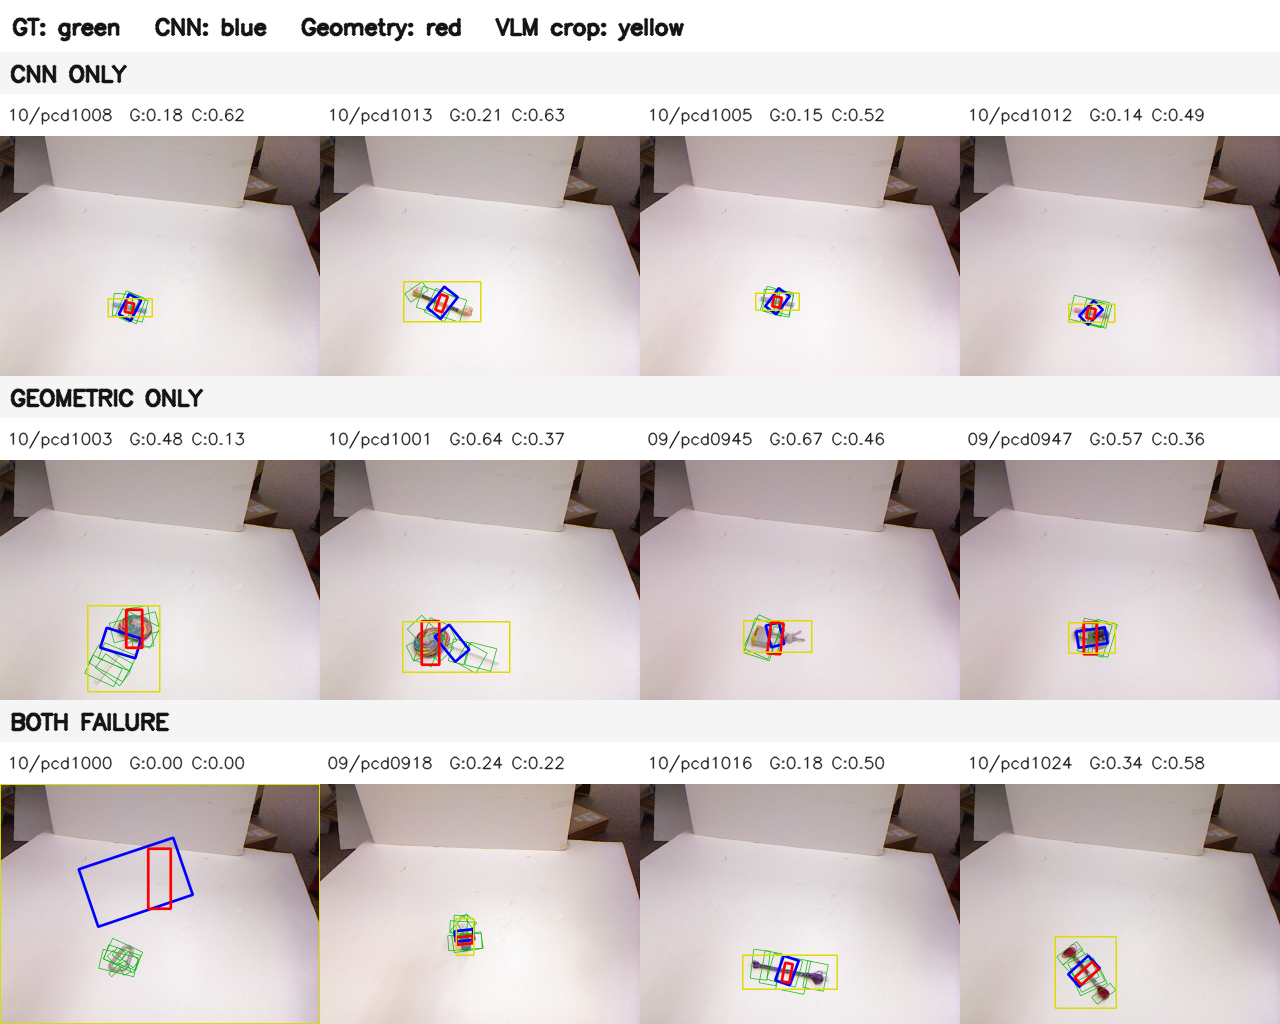
\includegraphics[width=\linewidth]{images/backend_failure_cases.png}
  \caption{Representative paired failures on the fixed test subset: CNN-only
  successes, geometry-only successes, and failures shared by both backends.
  Samples were selected by outcome category to expose complementarity and
  common limitations, not to estimate category frequency visually.}
  \label{fig:backend-failures}
\end{figure}

\section{Comparative Analysis}
The whole-dataset comparison supports a strong but bounded conclusion:
constraining the existing colour/contour estimator with open-vocabulary
localisation is more effective than applying it to the whole image. This is
supported by success rate, IoU, angle error, and elimination of missing-contour
predictions. It does not isolate whether Grounding DINO is superior to every
possible conventional detector.

The paired test analysis further divides the 85 images into 52 cases where both
backends succeed, 16 where only the CNN succeeds, 12 where only geometry
succeeds, and five where both fail. Thus, neither local backend strictly
dominates the other: 28 images produce a discordant binary outcome. The CNN's
higher IoU and the geometric backend's lower angle error are consistent with
this complementarity. A future hybrid could retain the geometric orientation
prior while learning centre and scale, but that hypothesis is not tested in the
current results.

The test subset scores must be interpreted alongside the split audit. Because
even the traditional baseline performs much better on directories 09--10 than
on directories 01--06, the CNN's higher fixed-test result is not evidence that
unseen objects are generally easier or that the model has achieved broad
object-level generalisation. The defensible finding is narrower: on these same
85 images and this evaluation implementation, the saved CNN run succeeds four
times more often than the geometric backend.

%==============================================================================
\chapter{General Discussion}

\section{Summary and Interpretation of Findings}
The strongest result is the improvement obtained by adding the Grounding DINO
front end to an otherwise similar geometric estimator. Whole-dataset success
increases by 16.38 percentage points, from 56.95\% to 73.33\%, while missing
predictions fall from 55 to zero. This indicates that, in the controlled
Cornell setting, restricting segmentation and contour selection to a
language-grounded region is more consequential than changing the local backend
from geometry to the current CNN. The finding concerns this generic prompt and
baseline; it does not establish that a VLM is necessary when a strong
task-specific detector is available.

The learned backend produces the highest whole-dataset mean IoU
($0.4510\pm0.0081$), suggesting that it estimates grasp centre and extent more
closely than fixed short-side rules. In contrast, the geometric backend has the
lowest mean angle error ($14.81^\circ$ over all images and $12.01^\circ$ on the
fixed test subset). Its rule of orienting a grasp perpendicular to the object
long axis is therefore still a useful prior. The two properties should not be
collapsed into the binary Cornell score: CNN improvements are mainly spatial,
whereas geometry remains more stable in orientation.

The paired test outcomes reinforce this interpretation. Sixteen images are
successful only for the CNN and 12 only for geometry. These 28 discordant cases
show that the two backends are complementary rather than ordered versions of
one another. A hybrid that learns centre and size while regularising direction
with a geometric prior is a plausible next experiment, but the current evidence
does not show that it would improve the combined criterion.

Finally, the apparent strength of the 85-image test result is constrained by
the split audit. The non-learning traditional baseline rises from 53.17\% on
training directories to 74.12\% on test directories. Since model generalisation
cannot cause this increase, directory composition or difficulty is a credible
confounder. The test result is therefore evidence about a fixed paired subset,
not a general object-wise generalisation claim.

\section{Relationship to Previous Literature}
The project follows the established Cornell rectangle formulation
\citep{jiang2011efficient} and its IoU-and-angle success criterion, but its
reported values are not directly interchangeable with standard Cornell
leaderboards. Lenz et al.\ use RGB-D input and image-wise/object-wise evaluation
\citep{lenz2015deep}; Redmon and Angelova also include depth and report standard
five-fold results for global and multi-grasp regression
\citep{redmon2015real}. Kumra and Kanan employ a substantially larger RGB-D
ResNet-based model \citep{kumra2017robotic}. In contrast, this study uses RGB
VLM crops and a directory-based split.

More recent work also changes the output representation. GG-CNN predicts grasp
quality, angle, and width at every depth pixel
\citep{morrison2018closing}; GR-ConvNet and Gaussian-guided generative networks
continue this dense grasp-map direction
\citep{kumra2020antipodal,li2022gaussian}. Their higher reported Cornell
accuracies contextualise the limited capacity of a single global rectangle
regressor, but do not form a fair numerical ranking because input modalities,
splits, augmentation, and output multiplicity differ. Park et al.'s 2018
high-resolution FCNN preprint is additionally excluded from the main comparison
because that version was withdrawn and superseded.

The language-conditioned role is closer in motivation to recent
language-driven grasp detection \citep{vuong2024language}, but the tasks remain
different. Grasp-Anything++ conditions grasp generation on object-specific
instructions in complex scenes, whereas the present prompt is the same generic
\texttt{small object} phrase for single-object Cornell images. The contribution
here is consequently a modular evaluation of open-vocabulary localisation as a
front end, not a new language-driven grasp benchmark.

Offline rectangle accuracy must also be separated from physical grasp success.
Physical experiments reported by GG-CNN and GR-ConvNet include sensing,
calibration, motion, contact, and recovery. A rectangle passing the Cornell
metric verifies only image-plane agreement with an annotation; it cannot be
compared directly with a percentage of objects successfully lifted by a robot.

\section{Failure Case Analysis}
The earlier whole-dataset geometric analysis separates its 236 failures into
126 IoU-only failures, 45 angle-only failures, and 65 failures of both
conditions. These are observed metric categories, not automatically causal
diagnoses. In particular, a 100\% localisation coverage rate means only that
Grounding DINO returned a box; it does not prove that every box tightly and
correctly localised the object.

The representative cases in Figure~\ref{fig:backend-failures} were chosen by a
fixed metric rule. For CNN-only samples 10/pcd1008, 10/pcd1013, 10/pcd1005, and
10/pcd1012, the geometric rectangles have IoU between 0.145 and 0.206, while
the CNN rectangles reach 0.489--0.627. The observed result is that the learned
rectangles better match annotated extent. A possible explanation is that the
contour short-side heuristic underestimates grasp size on these objects;
confirming that explanation would require an explicit component ablation.

The geometry-only row contains two distinct observations. On 10/pcd1003 the
CNN has low IoU (0.127), whereas on 10/pcd1001, 09/pcd0945, and 09/pcd0947 its
angle error exceeds the $30^\circ$ threshold. The latter is consistent with
unstable orientation regression, while the former is a spatial error. It would
be inaccurate to assign one common cause to all four cases.

The shared failures are similarly heterogeneous. Sample 10/pcd1000 has a
near-full-image VLM box and zero IoU for both backends, so poor localisation is
a plausible upstream contributor. Sample 09/pcd0918 is instead a borderline
size/position failure: both angle errors are below $4^\circ$, but both IoUs are
just below 0.25. Samples 10/pcd1016 and 10/pcd1024 have adequate CNN IoU but
angle errors above $74^\circ$, isolating orientation as the observed failure.
This case-level separation motivates treating centre/size and direction as
distinct learning targets.

\section{Practical and Theoretical Implications}
Practically, an open-vocabulary detector can serve as a replaceable perception
module that narrows the search space for a lightweight grasp estimator. This is
useful when object names vary or a closed-set detector is unavailable. The
results also argue for retaining simple geometric information: learned spatial
regression and analytic orientation priors solve different subsets of cases.

Theoretically, the experiment supports a modular account of error. Language
grounding addresses target selection, while grasp geometry addresses
affordance. Strong coverage in the first module does not imply success in the
second. This distinction is important when evaluating foundation models in
robotics: semantic localisation can improve a pipeline without itself learning
contact mechanics or manipulation.

For deployment, the next system stages would be depth recovery, camera-to-robot
calibration, pre-grasp planning, close-range re-estimation, gripper closure, and
success detection. The current offline output is best understood as an input to
those stages, not as a complete robotic grasping system.

\section{Limitations}
The study has seven principal limitations. First, evaluation uses only Cornell,
whose mostly uncluttered tabletop images do not represent open-world scenes.
Second, the paired test subset contains only 85 images, so four additional
successes correspond to 4.71 percentage points. Third, the directory split is
not a standard object-wise protocol, and the split audit indicates unequal
difficulty. Fourth, both backends emit only one grasp and cannot represent
multiple valid grasp modes.

Fifth, Grounding DINO's 885/885 coverage is not a localisation-accuracy metric;
a loose or incorrect box can still count as detected. Sixth, the study performs
no physical robot execution, so it does not measure collision-free reachability,
gripper contact, lifting, or recovery. Seventh, the CNN is trained on only 600
images and its five-run test success has a 4.53 percentage-point standard
deviation. Results are consequently sensitive to training randomness, and the
lightweight engineering choices should be interpreted as a baseline rather
than a settled architecture.

%==============================================================================
\chapter{Conclusion}

\section{Summary of the Dissertation}
\todo{Summarise the full dissertation: background, literature gap, methodology, experiments, results, and discussion.}

\section{Answers to the Research Questions}
\todo{Answer each research question clearly using evidence from the results and discussion.}

\section{Contributions and Practical Relevance}
\todo{State the final contributions and explain the real-world or practical relevance of the work.}

\section{Limitations and Recommendations}
\todo{Briefly restate the main limitations and provide recommendations for future work, such as real robot validation, stronger segmentation, larger datasets, and improved adaptation.}

%==============================================================================
\begin{appendices}

\chapter{Additional Material}

\section{Additional Figures}
The directory-balanced dataset contact sheet is provided in
Figure~\ref{fig:cornell-splits}, and the category-selected paired backend
examples are provided in Figure~\ref{fig:backend-failures}. The source records
used to regenerate these figures are
\path{representative_samples.csv} and
\path{sample_comparison.csv}, respectively.

\section{Additional Tables}
\begin{table}[htbp]
  \centering
  \caption{Success rate by fixed project split. The CNN row is the final saved
  seed-46 run and is used only for per-sample analysis.}
  \label{tab:split-success}
  \begin{tabular}{lrrr}
    \toprule
    Method & Train (600) & Validation (200) & Test (85) \\
    \midrule
    Traditional CV & 53.17\% & 61.00\% & 74.12\% \\
    VLM + geometric backend & 71.00\% & 79.50\% & 75.29\% \\
    VLM + CNN, seed 46 & 73.83\% & 73.50\% & 80.00\% \\
    \bottomrule
  \end{tabular}
\end{table}

\section{Configuration Details}
The original experiment environment was recorded as Conda environment
\texttt{msc-grasp} with PyTorch 2.5.1+\texttt{cu121}. The Grounding DINO
publisher was \texttt{IDEA-Research}, and the checkpoint was
\texttt{grounding-dino-tiny}. It used the generic prompt
\texttt{small object}, box threshold 0.25, and text threshold 0.25. The VLM box
was expanded by 10\% before local estimation.

The CNN used crop size 224, batch size 32, learning rate $10^{-3}$, weight decay
$10^{-4}$, a maximum of 80 epochs, and early-stopping patience 20. Repeated
runs used seeds 42--46.

\subsection*{Core commands}
\begin{lstlisting}
conda run -n msc-grasp python src/shared/check_cornell_dataset.py
conda run -n msc-grasp python src/baseline_cv/run_cv_baseline.py
conda run -n msc-grasp python \
  src/vlm/run_grounding_dino_localization.py --all --device cuda
conda run -n msc-grasp python src/vlm/run_vlm_assisted_grasp.py
conda run -n msc-grasp python \
  src/vlm/run_cnn_grasp.py --mode multi --num-runs 5 --device cuda
conda run -n msc-grasp python src/shared/analyze_cornell_splits.py
conda run -n msc-grasp python src/vlm/analyze_backend_comparison.py
\end{lstlisting}

\subsection*{Primary output files}
\begin{lstlisting}
data/processed/baseline_cv/cv_baseline_summary.json
data/processed/vlm/grasp/vlm_assisted_grasp_summary.json
data/processed/vlm/cnn_grasp/multi_run_summary.json
data/processed/vlm/cnn_grasp/cnn_grasp_predictions.csv
data/processed/shared/split_audit/split_metrics.json
data/processed/shared/split_audit/same_test_subset_metrics.csv
data/processed/vlm/backend_comparison/comparison_summary.json
data/processed/vlm/backend_comparison/sample_comparison.csv
\end{lstlisting}

The old 73.11\% CNN single-run value is not reproduced from these files and is
therefore excluded from the dissertation's primary evidence.

\end{appendices}

%==============================================================================
% The bibliography style is agsm (Harvard), as required by the template.
\bibliographystyle{agsm}
\renewcommand{\thechapter}{0}
\bibliography{l4proj}

\end{document}
